\documentclass{article}
\usepackage{fullpage}
\usepackage[utf8]{inputenc}
\usepackage{pict2e}
\usepackage{amsmath}
\usepackage{enumitem}
\usepackage{eurosym}
\usepackage{mathtools}
\usepackage{amssymb, amsfonts, latexsym, cancel}
\setlength{\parskip}{0.3cm}
\usepackage{graphicx}
\usepackage{fontenc}
\usepackage{slashbox}
\usepackage{setspace}
\usepackage{gensymb}
\usepackage{accents}
\usepackage{adjustbox}
\setstretch{1.35}
\usepackage{bold-extra}
\usepackage[document]{ragged2e}
\usepackage{subcaption}
\usepackage{tcolorbox}
\usepackage{xcolor, colortbl}
\usepackage{wrapfig}
\usepackage{empheq}
\usepackage{array}
\usepackage{parskip}
\usepackage{arydshln}
\graphicspath{ {images/} }
\renewcommand*\contentsname{\color{black}Índice} 
\usepackage{array, multirow, multicol}
\definecolor{lightblue}{HTML}{007AFF}
\usepackage{color}
\usepackage{etoolbox}
\usepackage{listings}
\usepackage{mdframed}
\setlength{\parindent}{0pt}
\usepackage{underscore}
\usepackage{hyperref}
\usepackage{tikz}
\usepackage{tikz-cd}
\usetikzlibrary{shapes, positioning, patterns}
\usepackage{tikz-qtree}
\usepackage{biblatex}
\usepackage{pdfpages}
\usepackage{pgfplots}
\usepackage{pgfkeys}
\addbibresource{biblatex-examples.bib}
\usepackage[a4paper, left=1cm, right=1cm, top=1cm,
bottom=1.5cm]{geometry}
\usepackage{titlesec}
\usepackage{titletoc}
\usepackage{tikz-3dplot}
\usepackage{kbordermatrix}
\usetikzlibrary{decorations.pathreplacing}
\newcommand{\Ej}{\textcolor{lightblue}{\underline{Ejemplo}}}
\setlength{\fboxrule}{1.5pt}

% Configura el formato de las secciones utilizando titlesec
\titleformat{\section}
{\color{red}\normalfont\LARGE\bfseries}
{Tema \thesection:}
{10 pt}
{}

% Ajusta el formato de las entradas de la tabla de contenidos
\addtocontents{toc}{\protect\setcounter{tocdepth}{4}}
\addtocontents{toc}{\color{black}}

\titleformat{\subsection}
{\normalfont\Large\bfseries\color{red}}{\thesubsection)}{1em}{\color{lightblue}}

\titleformat{\subsubsection}
{\normalfont\large\bfseries\color{red}}{\thesubsubsection)}{1em}{\color{lightblue}}

\newcommand{\bboxed}[1]{\fcolorbox{lightblue}{lightblue!10}{$#1$}}
\newcommand{\rboxed}[1]{\fcolorbox{red}{red!10}{$#1$}}

\DeclareMathOperator{\N}{\mathbb{N}}
\DeclareMathOperator{\Z}{\mathbb{Z}}
\DeclareMathOperator{\R}{\mathbb{R}}
\DeclareMathOperator{\Q}{\mathbb{Q}}
\DeclareMathOperator{\K}{\mathbb{K}}
\DeclareMathOperator{\im}{\imath}
\DeclareMathOperator{\jm}{\jmath}
\DeclareMathOperator{\col}{\mathrm{Col}}
\DeclareMathOperator{\fil}{\mathrm{Fil}}
\DeclareMathOperator{\rg}{\mathrm{rg}}
\DeclareMathOperator{\nuc}{\mathrm{nuc}}
\DeclareMathOperator{\dimf}{\mathrm{dimFil}}
\DeclareMathOperator{\dimc}{\mathrm{dimCol}}
\DeclareMathOperator{\dimn}{\mathrm{dimnuc}}
\DeclareMathOperator{\dimr}{\mathrm{dimrg}}
\DeclareMathOperator{\dom}{\mathrm{Dom}}
\DeclareMathOperator{\infi}{\int_{-\infty}^{+\infty}}
\newcommand{\dint}[2]{\int_{#1}^{#2}}

\newcommand{\bu}[1]{\textcolor{lightblue}{\underline{#1}}}
\newcommand{\lb}[1]{\textcolor{lightblue}{#1}}
\newcommand{\db}[1]{\textcolor{blue}{#1}}
\newcommand{\rc}[1]{\textcolor{red}{#1}}
\newcommand{\tr}{^\intercal}

\renewcommand{\CancelColor}{\color{lightblue}}

\newcommand{\dx}{\:\mathrm{d}x}
\newcommand{\dt}{\:\mathrm{d}t}
\newcommand{\dy}{\:\mathrm{d}y}
\newcommand{\dz}{\:\mathrm{d}z}
\newcommand{\dth}{\:\mathrm{d}\theta}
\newcommand{\dr}{\:\mathrm{d}\rho}
\newcommand{\du}{\:\mathrm{d}u}
\newcommand{\dv}{\:\mathrm{d}v}
\newcommand{\tozero}[1]{\cancelto{0}{#1}}
\newcommand{\lbb}[2]{\textcolor{lightblue}{\underbracket[1pt]{\textcolor{black}{#1}}_{#2}}}
\newcommand{\dbb}[2]{\textcolor{blue}{\underbracket[1pt]{\textcolor{black}{#1}}_{#2}}}
\newcommand{\rub}[2]{\textcolor{red}{\underbracket[1pt]{\textcolor{black}{#1}}_{#2}}}

\author{Francisco Javier Mercader Martínez}
\date{}
\title{Señales y Sistemas\\Problemas Unidad 3}

\begin{document}
\maketitle
\begin{enumerate}[label=\color{red}\textbf{\arabic*)}]
    \item \lb{Expresar la señal $x(t)=\sin(3\pi t)$ como una combinación lineal de exponenciales complejas.}

      \begin{minipage}{0.55\textwidth}
        $x(t)=\sin(3\pi t)=\begin{cases}
            \omega_0=3\pi\\
            T=\dfrac{2\pi}{\omega_0}=\dfrac{2\pi}{3\pi}=\dfrac{2}{3}
        \end{cases}$

        $\sin(3\pi x)=\dfrac{e^{j 3\pi t}-e^{-j 3\pi t}  }{2j}=\lbb{\dfrac{1}{2j}}{a_1}e^{j 3\pi t}-\lbb{\dfrac{1}{2j})}{a_{-1}}e^{-j 3\pi t}=\begin{cases}
            a_1=\dfrac{1}{2j}\\
            a_{-1}=-\dfrac{1}{2j}
        \end{cases}$
      \end{minipage}
      \begin{minipage}{0.35\textwidth}
          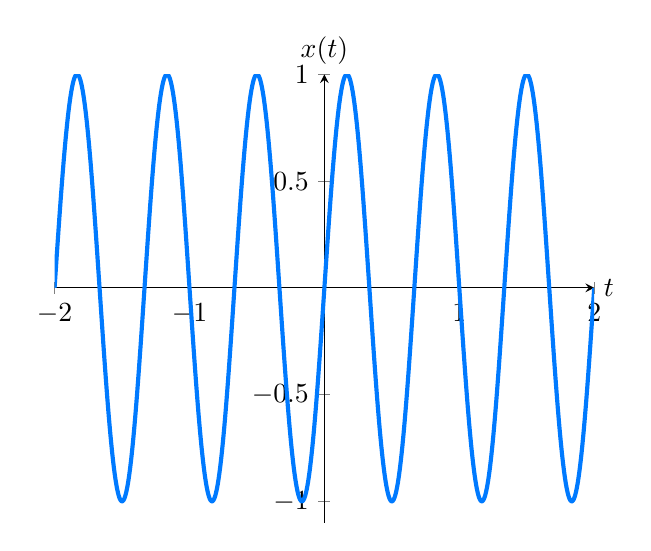
\begin{tikzpicture}
              \begin{axis}[
                  xmin= -2, xmax= 2,
                  ymin= -1.1, ymax = 1,
                  xlabel={$t$}, ylabel={$x(t)$},
                  axis lines = middle,
                  xlabel style={at={(axis cs:2,0)}, anchor=west},
                  ylabel style={at={(axis cs:0,1)}, anchor=south},
              ]
                  \addplot[domain=-2:2, samples=1000, lightblue, line width=1.5] {sin(deg(3*pi*x))};
              \end{axis}
          \end{tikzpicture}
      \end{minipage}
  \item \lb{Expresar la señal $x(t)=\sum_{n=-\infty}^{\infty} \prod\left( \dfrac{t-nT}{\tau} \right) $ como una combinación lineal de exponenciales complejas.}

$\omega_0=\dfrac{2\pi}{T}$

      $\begin{aligned}
          a_k & =\dfrac{1}{T}\int_{-\frac{T}{2} }^{\frac{T}{2} } \prod\left( \dfrac{t-nT}{\tau}\right)e^{-jk\omega_0 t}\dt=\dfrac{1}{T}\int_{-\frac{\tau}{2} }^{\frac{\tau}{2} } e^{-jk\omega_0t}\dt =\dfrac{1}{T}\cdot \left[ \dfrac{e^{-jk\omega_0t} }{-jk\omega_0} \right]_{-\frac{\tau}{2} }^{\frac{\tau}{2} }\\ 
              & =\dfrac{1}{T}\cdot \left[ \dfrac{e^{-jk\frac{2\pi}{T} t} }{-j\frac{2\pi}{T} } \right] _{-\frac{\tau}{2} }^{\frac{\tau}{2} }=\dfrac{1}{T}\cdot \left[\dfrac{e^{-jk\frac{\pi\tau}{T} } }{-jk\frac{2\pi}{T} }-\dfrac{e^{jk\frac{\pi\tau}{T} } }{-jk\frac{2\pi}{T} }  \right] =\dfrac{e^{jk\frac{\pi\tau}{T} } }{jk 2\pi}-\dfrac{e^{-jk\frac{\pi\tau}{T} } }{jk 2\pi}\\
              & =\dfrac{\sin\left( k\frac{\pi\tau}{T}  \right) }{\pi k}=\dfrac{\tau}{T}\cdot \dfrac{\sin\left( k\frac{\pi\tau}{T}  \right) }{k\frac{\pi\tau}{T} }=\dfrac{\tau}{T}\cdot \text{sinc}\left( \dfrac{k\tau}{T} \right) 
      \end{aligned}
      $

      $x(t)=\sum_k a_k\cdot e^{jk\frac{2\pi}{T} t} =\sum_k \dfrac{\tau}{T}\cdot \text{sinc}\left( \dfrac{k\tau}{T} \right) \cdot e^{jk\frac{2\pi}{T} t} $

      \begin{center}
      	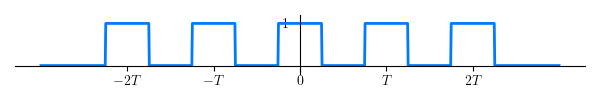
\includegraphics{Figure_1}
      \end{center}
      \newpage
  \item \lb{Calcular los coeficientes del desarrollo en series de Fourier: \[
  x(t)=A
  \] } 
\begin{center}
    \begin{tikzpicture}
        \begin{axis}[
            xmin= -5, xmax= 5,
            ymin= -0.1, ymax = 1.1,
            xlabel={$t$}, ylabel={$x(t)$},
            axis lines = middle,
            xlabel style={at={(axis cs:5,0)}, anchor=west},
            ylabel style={at={(axis cs:0,1.1)}, anchor=south},
            ytick={1},
            yticklabels={$A$}
        ]
            \addplot[domain=-5:5, samples=1000, lightblue, line width=1.5] {1};
        \end{axis}
    \end{tikzpicture}
\end{center}

  $\omega_0=\dfrac{2\pi}{T}$

  $a_k=\dfrac{1}{T}\cdot \int_{-\frac{T}{2} }^{\frac{T}{2} } A\cdot e^{-jk\omega_0t}\dt=\dfrac{A}{T}\cdot \left[ \dfrac{e^{-jk\frac{2\pi}{T} t} }{-jk\frac{1\pi}{T} } \right] _{-\frac{T}{2} }^{\frac{T}{2} }=\dfrac{A}{T}\cdot \left[ \dfrac{e^{-jk\pi} }{-jk\frac{2\pi}{T} }-\dfrac{e^{jk\pi} }{jk\frac{2\pi}{T} }  \right] =A\cdot \left( \dfrac{e^{jk\pi} }{jk 2\pi}-\dfrac{e^{-jk\pi} }{jk 2\pi} \right) =A\cdot \dfrac{\sin(k\pi)}{k\pi}=A\cdot \text{sinc}(k)  $

\item \lb{Calcular los coeficientes del desarrollo en series de Fourier: \[
x(t)=\sum_{n=-\infty}^{\infty} \delta(t-nT)
\] } 

\begin{center}
    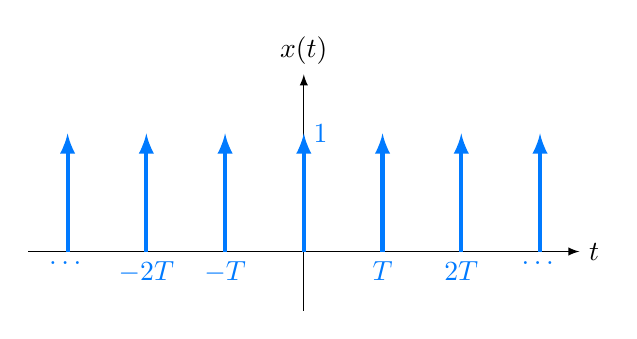
\begin{tikzpicture}[yscale=1.5]
        \draw[-latex] (-3.5,0) -- (3.5,0) node[right] {$t$};
        \draw[-latex] (0,-0.5) -- (0,1.5) node[above] {$x(t)$};
        \foreach \x in {-3,-2,...,3} {\draw[-latex, lightblue, line width=1.5] (\x,0) -- (\x,1);}
         \node[lightblue, right] at (0,1) {$1$};
         \foreach \x in {-3, 3} {\node[below, lightblue] at (\x,0) {$\dots$};}
         \foreach \x in {-2, 2} {\node[below, lightblue] at (\x,0) {$\x T$};}
             \node[below, lightblue] at (-1,0) {$-T$};
             \node[below, lightblue] at (1,0) {$T$};
    \end{tikzpicture}
\end{center}

$a_k=\dfrac{1}{T}\int_{-\frac{T}{2} }^{\frac{T}{2} } \delta(t)\cdot e^{-jk\frac{2\pi}{T} t}\dt=\left\{ \delta(t)\to t_0=0\to e^{-jk\frac{2\pi}{T}\cdot 0 }=1  \right\} =\dfrac{1}{T}\int_{-\frac{T}{2} }^{\frac{T}{2} } \delta(t)\dt=\dfrac{1}{T}   $

\item \lb{Calcular los coeficientes del desarrollo en series de Fourier:}
    \begin{center}
        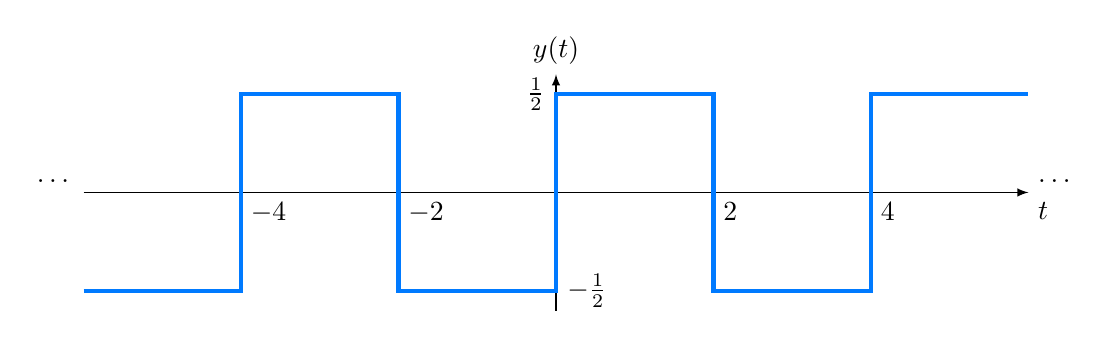
\begin{tikzpicture}[yscale=2.5]
            \draw[-latex] (-6, 0) node[above left] {$\dots$} -- (6,0) node[below right] {$t$} node[above right] {$\dots$};
            \draw[-latex] (0,-0.6) -- (0,0.6) node[above] {$y(t)$};
            \draw[lightblue, line width=1.5] (-6,-0.5) -- (-4,-0.5) -- (-4,0.5) -- (-2,0.5) -- (-2,-0.5) -- (0,-0.5) node[right,black] {$-\frac{1}{2}$} -- (0,0.5) node[left,black] {$\frac{1}{2}$} -- (2,0.5) -- (2,-0.5) -- (4,-0.5) -- (4,0.5) -- (6,0.5);
            \foreach \x in {-4, -2, 2, 4} {\node[below right] at (\x, 0) {$\x$};}
             
        \end{tikzpicture}
    \end{center}

    $\begin{aligned}
    a_k&=\dfrac{1}{4}\cdot \left( \int_{-2}^{0} -\dfrac{1}{2}\cdot e^{-jk\frac{\pi}{2} t} \dt+\int_{0}^{2} \dfrac{1}{2} \cdot e^{-jk\frac{\pi}{2}t}\dt\right)=\dfrac{1}{4}\cdot \left( \left[ -\dfrac{1}{2}\cdot \left( \dfrac{e^{0}}{jk\frac{\pi}{2} } -\dfrac{e^{jk\pi} }{-jk\frac{\pi}{2} }\right)  \right] +\left[ \dfrac{1}{2}\cdot \left( \dfrac{e^{-jk\pi} }{-jk\frac{\pi}{2} }-\dfrac{e^{0} }{-jk\frac{\pi}{2} } \right) \right]  \right)\\
       &=\dfrac{1}{8}\cdot \left( \dfrac{e^{0} }{jk\frac{\pi}{2} }- \dfrac{e^{jk\pi} }{jk\frac{\pi}{2} }-\dfrac{e^{-jk\pi} }{jk\frac{\pi}{2} }+\dfrac{e^{0} }{jk\frac{\pi}{2} }\right)=\dfrac{1}{8}\cdot \left( \dfrac{2-2\cdot (-1)^k}{jk\frac{\pi}{2} } \right) =\dfrac{1}{4}\cdot \dfrac{1-(-1)^k}{jk\frac{\pi}{2} }=\dfrac{1-(-1)^k}{jk2\pi}
\end{aligned}$
\newpage
\item \lb{Calcular los coeficientes del desarrollo en series de Fourier:}
    \begin{center}
        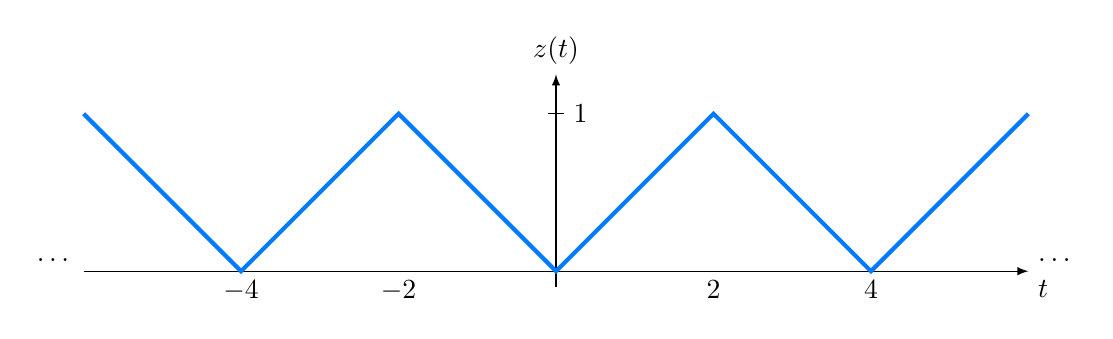
\begin{tikzpicture}[yscale=2]
            \draw[-latex] (-6, 0) node[above left] {$\dots$} -- (6,0) node[below right] {$t$} node[above right] {$\dots$};
            \draw[-latex] (0,-0.1) -- (0,1.25) node[above] {$z(t)$};
            \foreach \x in {-4, -2, 2, 4} {\node[below] at (\x, 0) {$\x$};}
                \draw[lightblue, line width=1.5] (-6,1) -- (-4,0) -- (-2,1) -- (0,0) -- (2,1) -- (4,0) -- (6,1); 
                \draw (-0.1,1) -- (0.1,1) node[right] {$1$};
        \end{tikzpicture}
    \end{center}
    $\frac{\partial }{\partial t} y(t)=x(t)\implies y(t)=\int_{-\infty}^{t} x(\tau) \mathrm{d}\tau$

    $y(t)\xrightarrow{DSF}\dfrac{a_k}{jk\omega_0}=\dfrac{1-(-1)^k}{\dfrac{jk 2\pi}{jk\frac{\pi}{2} }}=\dfrac{1-(-1)^k}{\dfrac{jk2\pi}{\frac{jk\pi}{2} }}=\dfrac{2-2(-1)^k}{-k^2\pi^22}=\dfrac{1-(-1)^k}{-k^2\pi^2}$ 
\item \lb{Calcular los coeficientes del desarrollo en series de Fourier:}
    \begin{center}
        \begin{tikzpicture}[xscale=2, yscale=1.5, >=latex]
            \draw[->] (-3,0) node[above left] {$\dots$} -- (3,0) node[below right] {$t$} node[above right] {$\dots$};
            \draw[->] (0,-1.3) -- (0,1.3) node[above] {$y(t)$};
            \foreach \y in {-1,1} {\draw (0.1,\y) -- (-0.1,\y) node[left] {$\y$};}
            \draw (-2,0.1) -- (-2,-0.1) node[below] {$-T$};
            \draw (2,0.1) -- (2,-0.1) node[below] {$T$};
            \draw[->, lightblue, line width=1.5] (-2.5,0) -- (-2.5,1);
             \draw[->, lightblue, line width=1.5] (-1.5,0) -- (-1.5,-1);
             \draw[->, lightblue, line width=1.5] (-0.5, 0) node[below] {$-\dfrac{\tau}{2}$}-- (-0.5, 1) ;
             \draw[->, lightblue, line width=1.5] (0.5,0) node[above] {$\dfrac{\tau}{2}$}-- (0.5,-1);
 \draw[->, lightblue, line width=1.5] (1.5,0) -- (1.5,1);
 \draw[->, lightblue, line width=1.5] (2.5,0) -- (2.5,-1);
        \end{tikzpicture}
    \end{center}
    $\begin{aligned}
        \sum_{n=-\infty}^{\infty} \delta\left(t-nT+\dfrac{\tau}{2}\right)-\delta\left( t-nT-\dfrac{\tau}{2} \right)\xrightarrow{DSF}\dfrac{1}{T}\cdot e^{jk\frac{2\pi}{T}\cdot \frac{\tau}{2}  } -\dfrac{1}{T}\cdot e^{-jk\frac{2\pi}{T} \cdot \frac{\tau}{2} }& =\dfrac{e^{jk\frac{\pi\tau}{T} } -e^{-jk\frac{\pi\tau}{T} } }{T}=\dfrac{1}{T}\cdot 2j\cdot \dfrac{e^{jk\frac{\pi\tau}{T} } -e^{-jk\frac{\pi\tau}{T} } }{2j}\\
                                                                                                                                                                                                                                                                                           &=\dfrac{2j}{T}\cdot \sin\left( k \dfrac{\pi}{T}\tau \right)
    \end{aligned}$
\item \lb{Calcular la potencia total de la señal: $x(t)=\sin(3\pi t)$} 

    $P_{\infty}=P_T=\dfrac{1}{T}\int_{-\frac{T}{2}}^{\frac{T}{2}}|x(t)|^2\dt=\dfrac{3}{2}\int_{-\frac{1}{3}}^{\frac{1}{3}}|\sin(3\pi t)|^2\dt \equiv\sum_{k=-\infty}^{\infty}|a_k|^2=\left|\dfrac{1}{2j}\right|^2+\left|-\dfrac{1}{2j}\right|^2=\dfrac{1}{2}W$

  \item \lb{}
\end{enumerate}
\end{document}
